%\documentclass{beamer}
%\usetheme{Pittsburgh} 
\documentclass{scrartcl}

\usepackage[utf8]{inputenc}
\usepackage{default}
\usepackage[procnames]{listings}
\usepackage{graphicx}
%\usepackage[toc,page]{appendix}
\usepackage{caption}
\usepackage{hyperref}
\usepackage{color}


%Bibliogrpahy?
\usepackage{bibentry}
%\nobibliography*
%\bibentry{ }


\begin{document}

\title{Assignment No. 1}
\subtitle{}
\author{
  Quignon, Christophe \\
  %Familyname, Name
} 
\date{\today}


\maketitle

\section{Read Chapter 1 from Haykin’s book; summarize or sketch your insights in mind-map or an outline or a summary.}

\begin{figure}
 \center
 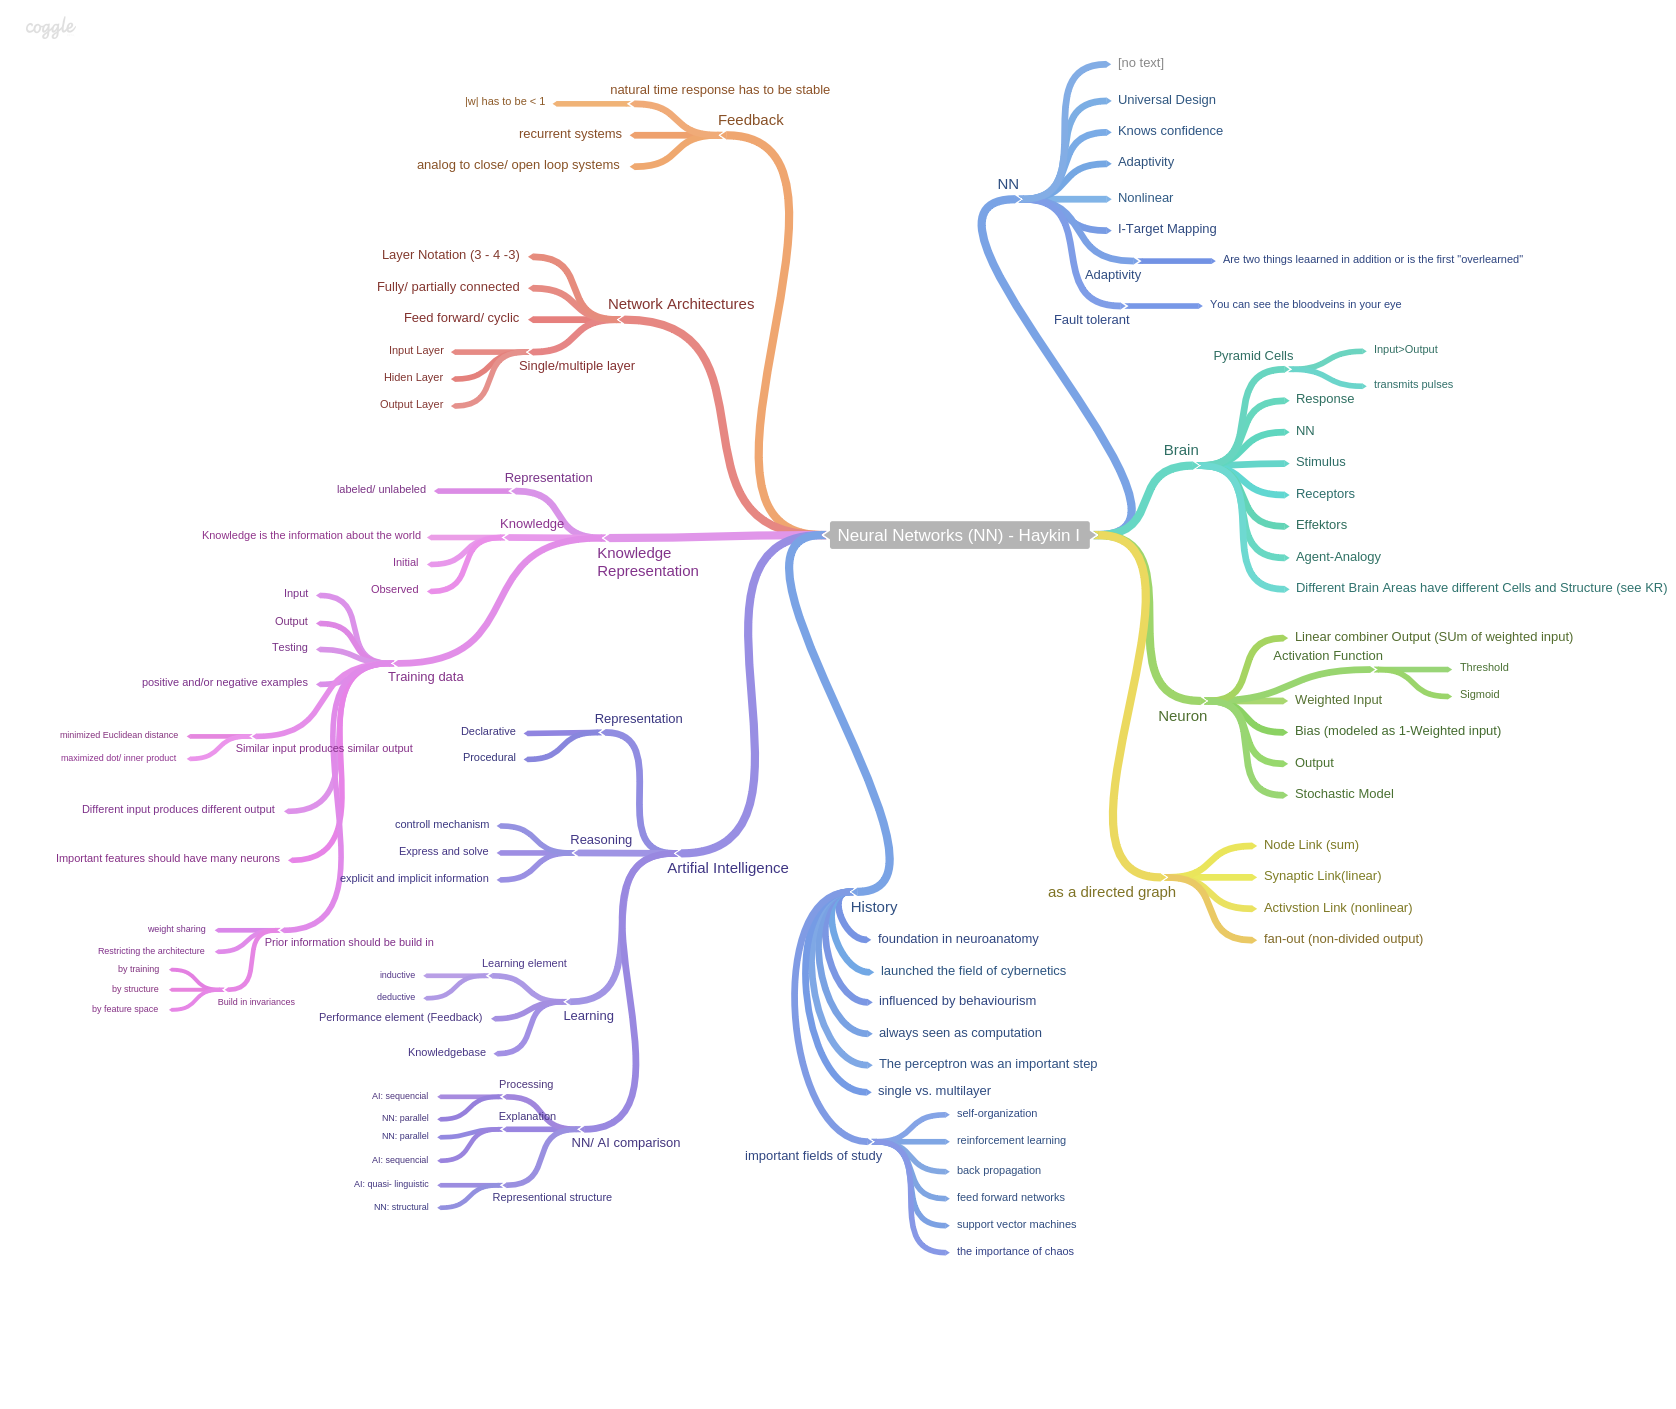
\includegraphics[width= \textwidth]{mindmap.png}
 \caption{Mindmap of chapter one}
 \label{fig:mindmap}
\end{figure}

See figure~\ref{fig:mindmap}.


\section{From Haykin’s book, Chapter 1 problems – “Models of a neuron”, solve any 2 out of 11
(1.1 to 1.11).
}
\subsection{1.9: A neuron j receives inputs from four other neurons whose activity levels are 10, -20, 4 and -2. The weights are 0.8, 0.2, -1.0, and -0.9. The bias is zero.}
\subsubsection{Calculate the output if the neuron is linear.}
$u_{k}=10*0.8-20*0.2+4*-1.0-2*-0.9=1.8$\\

\subsection{The neuron is represented by the McCulloch-Pits model.}
$y_{k}=\varphi(1.8+0)=1$\\

\subsection{1.10 Repeat the Problem from 1.9 with the logistic function.}
$\varphi (v)=1/(1+exp(-v))$\\
$\varphi (v)=1/(1+exp(-1.8))$\\
$\varphi (v)= -0.2568$

\section{From Haykin’s book, Chapter 1 problems – “Network architectures”, solve any 2 out of 7
(1.12 to 1.19) including 1.13.
}
\subsection{1.12 A fully connected feedforward network has 10 source nodes, 2 hidden layers, one with 4 neurons and one with 3 neurons, and a single output neuron. Construct an architectural graph of this network.}

\begin{figure}[p, b]
 \center
 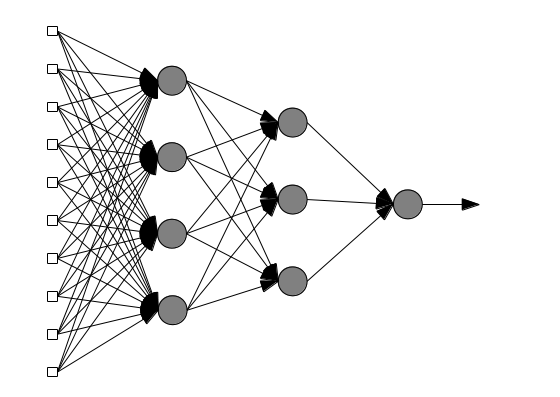
\includegraphics[width= \textwidth]{10-4-3-1-NN.png}
 \caption{Graph of a fully connected 10-4-3-1 neuronal network.}
 \label{fig:graph}
\end{figure}

See figure~\ref{fig:graph}.

\subsection{1.13}
\subsubsection{Input output mapping from the network from Figure 1.13 with a logistic function:}
$v_{3} = 1/(1+exp(-(5v_{1}+v_{2})))\\
v_{4} = 1/(1+exp(-(v_{1}-3v_{2})))\\
v_{5}= 1/(1+exp(-(3v_{3}-1v_{4})))\\
v_{6}=1/(1+exp(-(4v_{3}+6v_{4})))\\
v_{7}=1/(1+exp(-(-2v_{5}+v_{6})))\\
u_{k}=\varphi(v_{7})+b_{k}$\\

\subsubsection{Input output mapping from the network from Figure 1.13, supposed to operate in linear region.}
$v_{3} = 5v_{1}+v_{2}\\
v_{4}=2v_{1}-3v_{2}\\
v_{5}=3v_{3}-v_{4}\\
v_{6}=4v_{3}+6v_{4}\\
v_{7}=-2v_{5}+v_{6}$\\
$u_{k}=\varphi(6v_{1} - 26v_{2})+b_{k}$

\section{Optional: Solve 1.20 or 1.21 in section “Knowledge representation”
}
-


%CONTENTS
%NOTES


%COPY AND PASTE FROM HERE

%\begin{enumerate}
% \item 
%\end{enumerate}

%\hyperref{link}{text}

%\begin[Language=Python]{lstlisting}
%#PYTHON CODE HERE
%\end{lstlisting}

%\lstinputlisting[Language=Python]{ }

%\begin{figure}
% \center
% \includegraphics[width= cm]{ }
% \caption{}
%\end{figure}

%BIBLIOGRPAHY?
\bibliographystyle{plain}%amsalpha
\bibliography{Top30.bib}
%\bibentry{}

\end{document}
